\subsubsection{UC5 - Generazione prompt}\label{UC5}

\begin{figure}[H]
  \centering
  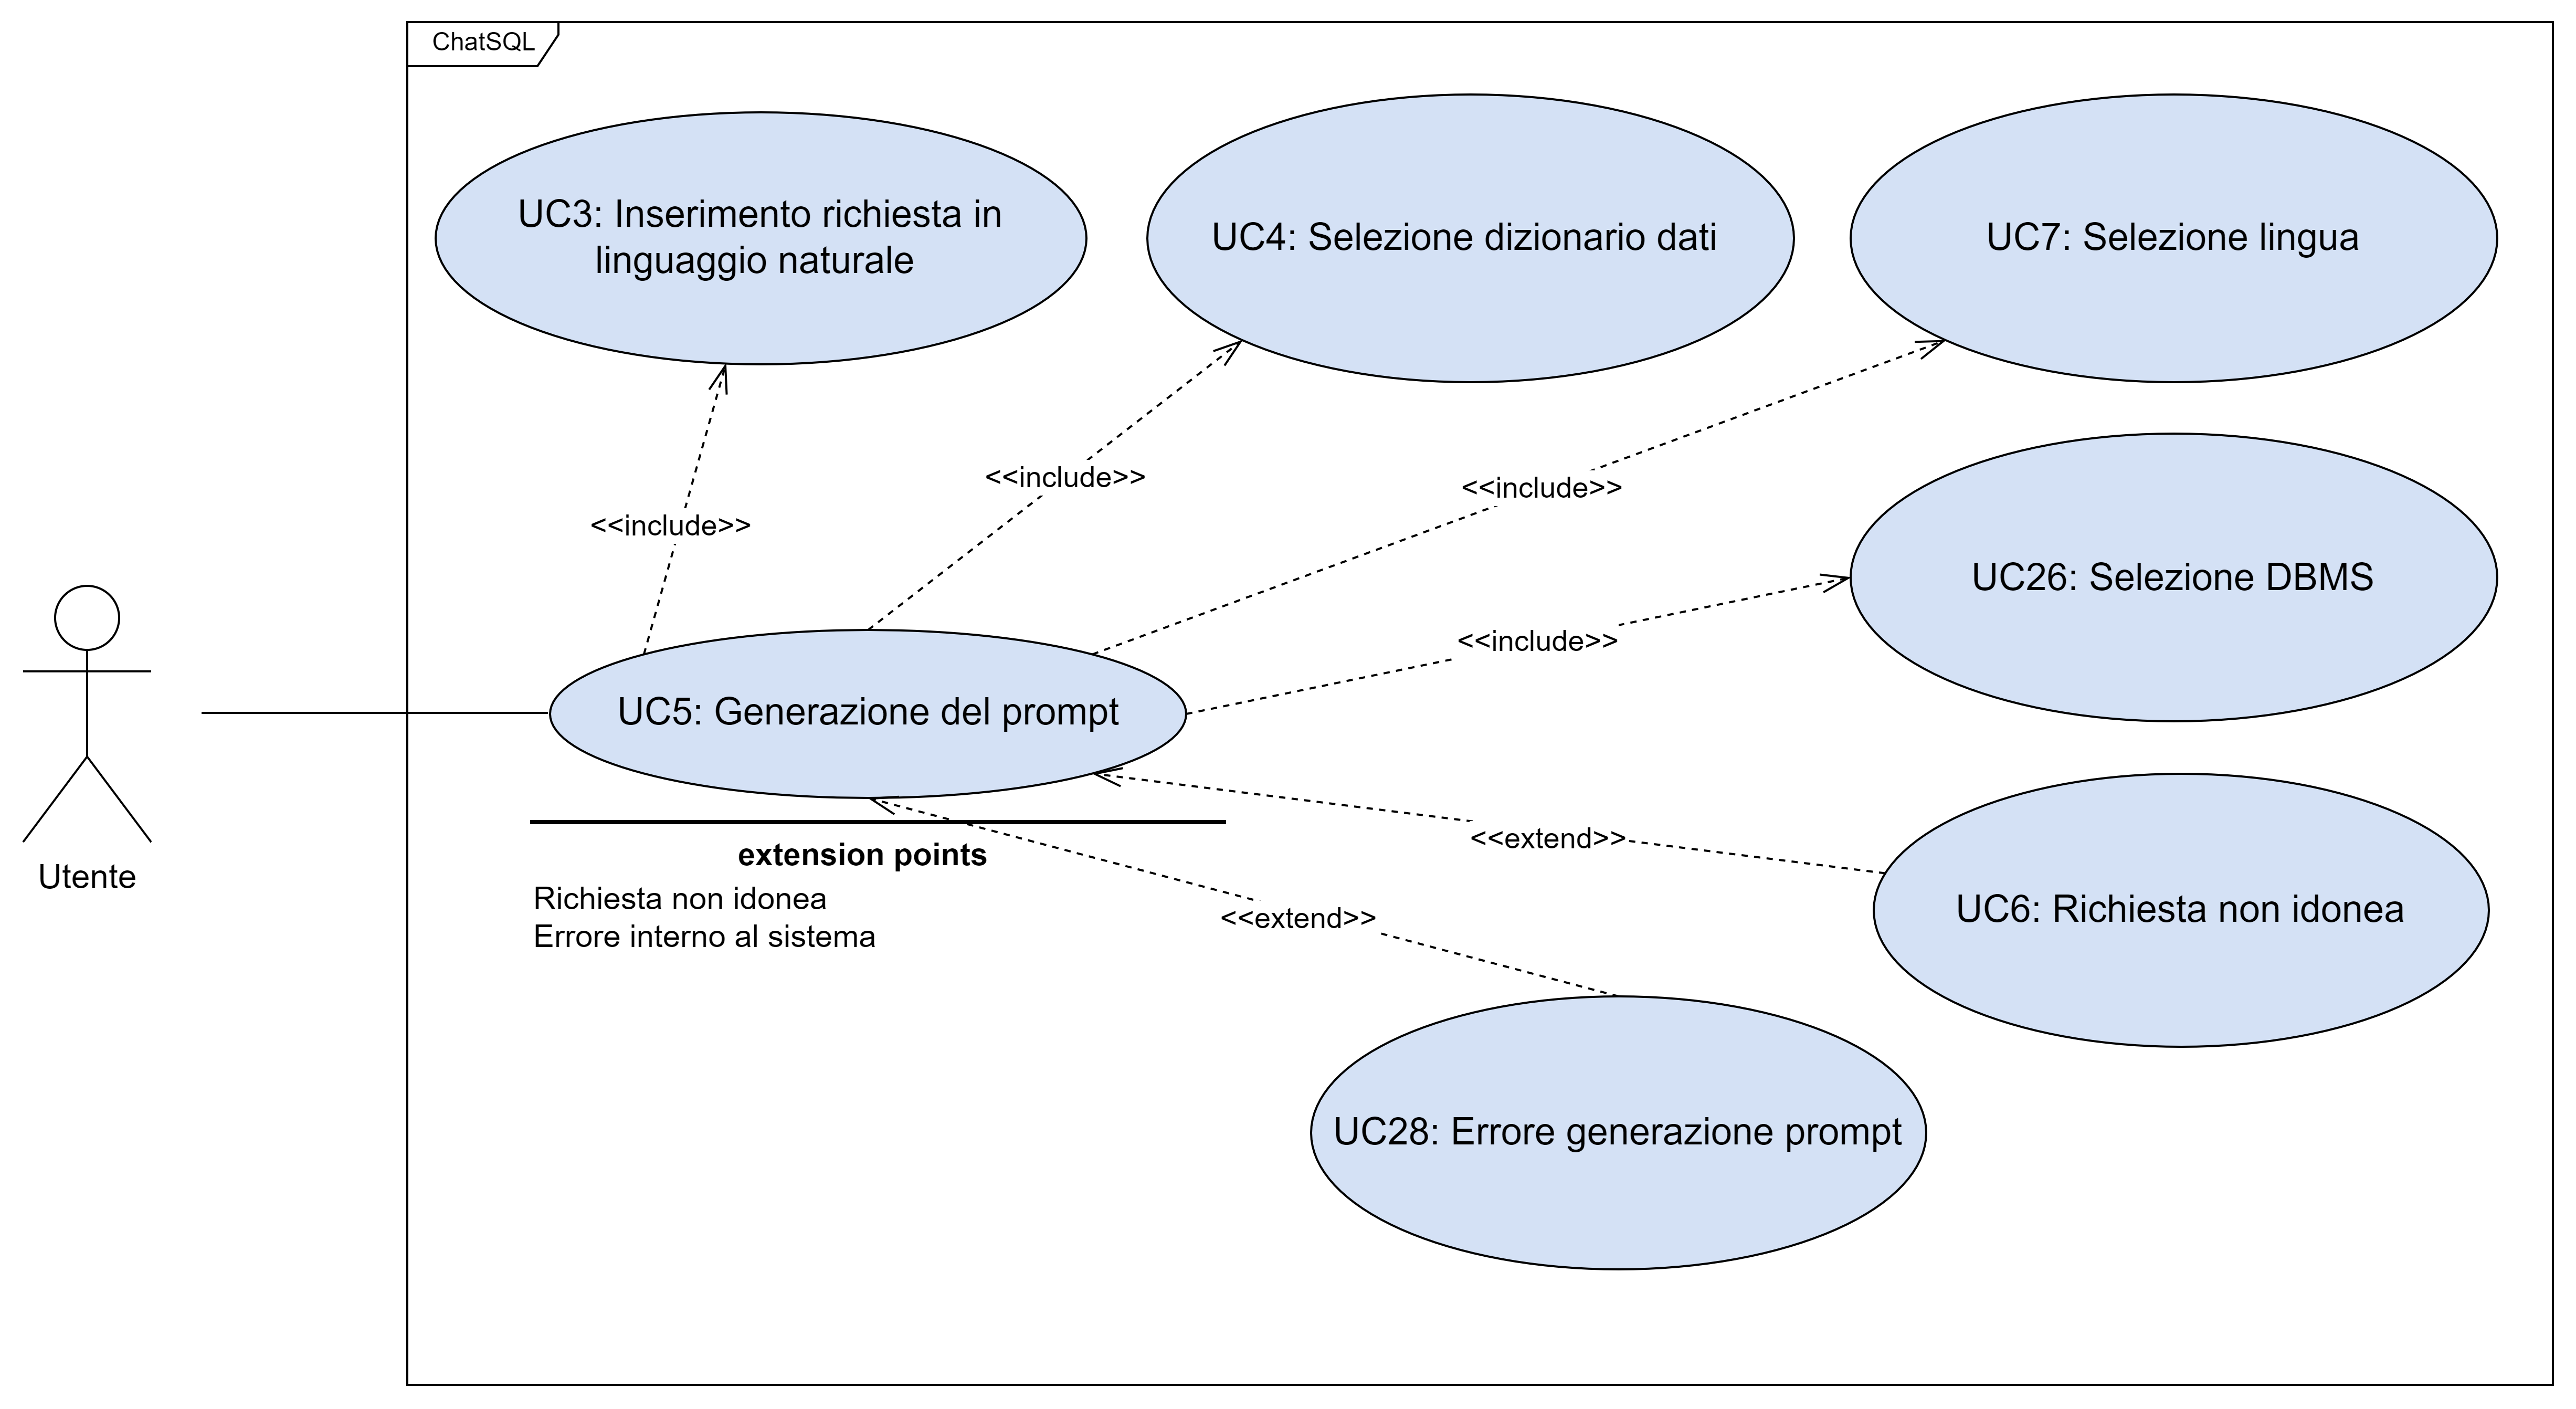
\includegraphics[width=0.90\textwidth]{assets/uc5.png}
  \caption{UC5}
\end{figure}

\paragraph*{Descrizione}
Il sistema genera un \glossario{prompt} a partire da una richiesta dell'Utente. Per comporre il \glossario{prompt}, il sistema cerca delle corrispondenze tra la richiesta e il \glossario{dizionario dati} selezionato. Il prompt generato può essere usato in combinazione con un modello di \glossario{AI} esterno per costruire \glossario{query} SQL.

\paragraph*{Attori principali}
Utente

\paragraph*{Precondizioni}
\begin{itemize}
  \item L'applicazione è stata avviata con successo;
  \item È presente almeno un \glossario{dizionario dati} nel sistema;
  \item È stato creato almeno un \glossario{indice vettoriale} per la ricerca semantica.
\end{itemize}

\paragraph*{Postcondizioni}
\begin{itemize}
  \item Il sistema ritorna con successo il \glossario{prompt} generato. Il prompt contiene i \glossario{metadati} estratti dal \glossario{dizionario dati}.
\end{itemize}

\paragraph*{Trigger}
L'Utente desidera ricevere un \glossario{prompt} in risposta alla sua richiesta.

\paragraph*{Scenario principale}
\begin{enumerate}
  \item L'Utente seleziona un \glossario{dizionario dati}(\hyperref[UC4]{UC4});
  \item L'Utene seleziona un \glossario{DBMS} (\hyperref[UC26]{UC26});
  \item L'Utente seleziona una lingua (\hyperref[UC7]{UC7});
  \item L'Utente inserisce una richiesta in linguaggio naturale (\hyperref[UC3]{UC3});
  \item L'Utente richiede la generazione del \glossario{prompt};
  \item Se l'Utente che ha effettuato la richiesta è un Tecnico, il sistema genera un file di \glossario{log} che documenta il processo di generazione del \glossario{prompt};
  \item Viene avviato il processo di generazione del \glossario{prompt};
  \item Il sistema restituisce il \glossario{prompt} generato.
\end{enumerate}

\paragraph*{Inclusioni}
\begin{itemize}
  \item Selezione \glossario{dizionario dati} (\hyperref[UC4]{UC4});
  \item Inserimento richiesta in linguaggio naturale (\hyperref[UC3]{UC3});
  \item Selezione lingua (\hyperref[UC7]{UC7});
  \item Selezione DBMS (\hyperref[UC26]{UC26}).
\end{itemize}

\paragraph*{Estensioni}
\begin{itemize}
  \item Visualizzazione avviso richiesta non idonea (\hyperref[UC6]{UC6}).
  \begin{itemize}
    \item Extension point: richiesta non idonea per il modello di \glossario{AI} o per il \glossario{dizionario dati} scelto.
  \end{itemize}
  \item Visualizzazione errore generazione del \glossario{prompt} (\hyperref[UC11]{UC11}).
    \begin{itemize}
      \item Extension point: errore interno al sistema.
    \end{itemize}
\end{itemize}